% !TeX root = ../analisi_2.tex

\section{Curve (\texorpdfstring{$\mathbb{R} \to \mathbb{R}^n$}{R to R n})}

\subsection{Definizioni ed esempi}

\begin{definition}
Sia $\varphi : [a, b] \to \mathbb{R}^n$ che a $t \in [a, b] \to \varphi(t) = (x_1(t), \dots, x_n(t)) \in \mathbb{R}^n$ dove $x_i(t) : [a, b] \to \mathbb{R}$ continua, $i = 1, \dots, n$, allora diremo che $\varphi$ è continua \pencilnote{(in $\mathbb{R}^2$ $\varphi(t) = (x(t), y(t))$).}

Allora $\varphi$ si chiama \underline{curva}.
\end{definition}

Le equazioni
\[
\varphi : \begin{cases}
x_1 = x_1(t) \\
x_2 = x_2(t) \\
\vdots \\
x_n = x_n(t)
\end{cases} \quad t \in [a, b]
\]
si chiamano eq. param. della curva e si possono anche scrivere in riga: $\varphi(t) = (x_1(t), \dots, x_n(t))$.

Si chiama \underline{sostegno} della curva il suo \underline{codominio}.

I punti $\varphi(a)$ e $\varphi(b)$ si chiamano punto iniziale e punto finale della curva.

Una curva si dice \underline{chiusa} se $\varphi(a) = \varphi(b)$.

\begin{example}
$\varphi_1 : [0, 2\pi] \to \varphi_1(t) = (\cos t, \sin t)$ chiusa

$\varphi_2 : [0, 3\pi] \to \varphi_2(t) = (\cos t, \sin t)$ non chiusa

\begin{center}
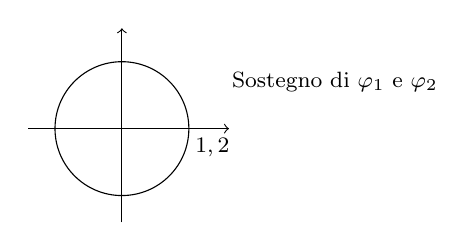
\begin{tikzpicture}[scale=0.85]
    \draw[->] (-1.4,0) -- (1.6,0);
    \draw[->] (0,-1.4) -- (0,1.5);
    \draw (0,0) circle (1);
    \node[below right] at (0.95,0) {\footnotesize $1, 2$};
    \node[right] at (1.5,0.7) {\footnotesize Sostegno di $\varphi_1$ e $\varphi_2$};
\end{tikzpicture}
\end{center}
\end{example}

\begin{oss}
Due curve che hanno lo stesso sostegno, non sono necessariamente la stessa curva!
\end{oss}

\begin{definition}
Una curva $\varphi : [a, b] \to \mathbb{R}^n$ si dice \underline{semplice} se $\forall t_1 \neq t_2$, con almeno uno dei due interno ad $[a, b]$, risulta $\varphi(t_1) \neq \varphi(t_2)$.
\end{definition}

\begin{oss}
Le chiuse possono essere semplici.
\end{oss}

\begin{definition}
Una curva $\varphi : [a, b] \to \mathbb{R}^n$ si dice \underline{regolare} se:
\begin{enumerate}
    \item $\varphi \in C^1([a, b])$
    \item posto $\varphi'(t) = (x'_1(t), \dots, x'_n(t)) \neq (0, \dots, 0)$ ovvero $\vert \varphi'(t) \vert > 0 \quad \forall t \in ]a, b[$
\end{enumerate}
\end{definition}

$\varphi'(t)$ si chiama vettore tangente alla curva ed il versore tangente è:
\[
T(t) = \frac{\varphi'(t)}{\vert \varphi'(t) \vert}
\]

\begin{center}
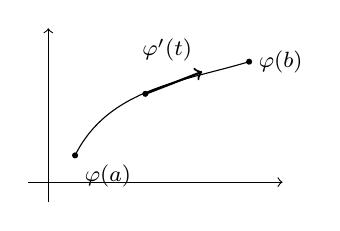
\begin{tikzpicture}[scale=0.85]
    \draw[->] (-0.3,0) -- (3.5,0);
    \draw[->] (0,-0.3) -- (0,2.3);
    \draw (0.4,0.4) .. controls (0.9,1.4) and (2.0,1.5) .. (3.0,1.8);
    \fill (0.4,0.4) circle (1.3pt) node[below right] {\footnotesize $\varphi(a)$};
    \fill (3.0,1.8) circle (1.3pt) node[right] {\footnotesize $\varphi(b)$};
    \fill (1.45,1.32) circle (1.3pt);
    \draw[->, thick] (1.45,1.32) -- (2.3,1.65) node[above left] {\footnotesize $\varphi'(t)$};
\end{tikzpicture}
\end{center}

\pencilnote{Oss.: posso vedere le funz. come curve $\varphi = (x, f(x))$.}

\begin{example}[Curve cartesiane]
Sia $f : [a, b] \to \mathbb{R}$, $f \in C^1([a, b])$.

Si chiama curva cartesiana la seg.:
\[
\varphi : t \in [a, b] \to \varphi(t) = (t, f(t)) \in \mathbb{R}^2
\]
\[
\varphi : \begin{cases}
x = t \\
y = f(x)
\end{cases}
\]
Osserviamo che il sostegno è il grafico di $f$.

\begin{center}
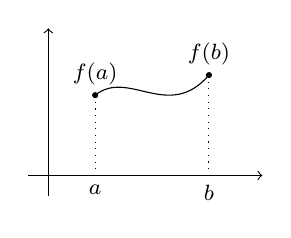
\begin{tikzpicture}[scale=0.85]
    \draw[->] (-0.3,0) -- (3.2,0);
    \draw[->] (0,-0.3) -- (0,2.2);
    \draw (0.7,1.2) .. controls (1.2,1.6) and (1.8,0.8) .. (2.4,1.5);
    \fill (0.7,1.2) circle (1.3pt) node[above] {\footnotesize $f(a)$};
    \fill (2.4,1.5) circle (1.3pt) node[above] {\footnotesize $f(b)$};
    \draw[dotted] (0.7,1.2) -- (0.7,0) node[below] {\footnotesize $a$};
    \draw[dotted] (2.4,1.5) -- (2.4,0) node[below] {\footnotesize $b$};
\end{tikzpicture}
\end{center}

Oss.:
\begin{enumerate}
    \item non è chiusa
    \item è semplice
    \item è regolare:
    \[
    \begin{cases}
    \varphi'(t) = (1, f'(t)) \\
    \vert \varphi'(t) \vert = \sqrt{1 + f'^2(t)} > 0 \quad \forall t \in [a, b]
    \end{cases}
    \]
\end{enumerate}
\end{example}

\begin{example}
Sia $\varphi(t) : [0, 2\pi] \to \mathbb{R}^2$ definita da
\[
\varphi : \begin{cases}
x(t) = x_0 + R \cos t \\
y(t) = y_0 + R \sin t
\end{cases} \quad t \in [0, 2\pi]
\]
dove $(x_0, y_0) \in \mathbb{R}^2$ e $R > 0$.

Il sostegno è:
\begin{center}
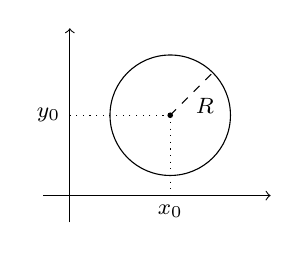
\begin{tikzpicture}[scale=0.85]
    \draw[->] (-0.4,0) -- (3.0,0);
    \draw[->] (0,-0.4) -- (0,2.5);
    \draw (1.5,1.2) circle (0.9);
    \fill (1.5,1.2) circle (1.2pt);
    \draw[dotted] (1.5,1.2) -- (1.5,0) node[below] {\footnotesize $x_0$};
    \draw[dotted] (1.5,1.2) -- (0,1.2) node[left] {\footnotesize $y_0$};
    \draw[dashed] (1.5,1.2) -- ({1.5 + 0.9*cos(45)}, {1.2 + 0.9*sin(45)}) node[midway, below right=-2pt] {\footnotesize $R$};
\end{tikzpicture}
\end{center}
\begin{enumerate}
    \item è chiusa
    \item è semplice
    \item è regolare: $\varphi'(t) = (-R \sin t, R \cos t)$, $\vert \varphi'(t) \vert = R > 0 \quad \forall t \in ]0, 2\pi[$
\end{enumerate}
\end{example}

\begin{example}
Sia $\varphi(t) : [0, 2\pi] \to \mathbb{R}^2$ def. come segue:
\[
\varphi(t) = \begin{cases}
x(t) = x_0 + a \cos t \\
y(t) = y_0 + b \sin t
\end{cases} \quad t \in [0, 2\pi]
\]
dove $(x_0, y_0) \in \mathbb{R}^2$ e $a, b > 0$ si dicono semiassi.

Il sostegno è:
\begin{center}
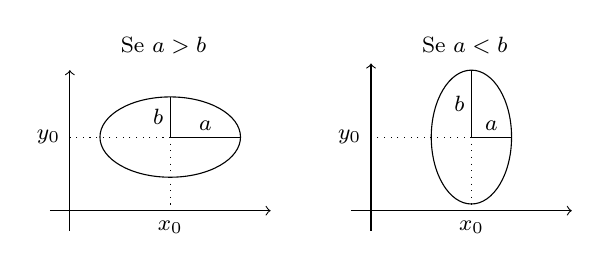
\begin{tikzpicture}[scale=0.85]
    % Se a > b
    \node[above] at (1.4,2.2) {\footnotesize Se $a > b$};
    \draw[->] (-0.3,0) -- (3.0,0);
    \draw[->] (0,-0.3) -- (0,2.1);
    \draw (1.5,1.1) ellipse (1.05 and 0.6);
    \draw[dotted] (1.5,1.1) -- (1.5,0) node[below] {\footnotesize $x_0$};
    \draw[dotted] (1.5,1.1) -- (0,1.1) node[left] {\footnotesize $y_0$};
    \draw (1.5,1.1) -- (2.55,1.1) node[midway, above=-1pt] {\footnotesize $a$};
    \draw (1.5,1.1) -- (1.5,1.7) node[midway, left=-1pt] {\footnotesize $b$};

    % Se a < b
    \begin{scope}[xshift=4.5cm]
        \node[above] at (1.4,2.2) {\footnotesize Se $a < b$};
        \draw[->] (-0.3,0) -- (3.0,0);
        \draw[->] (0,-0.3) -- (0,2.2);
        \draw (1.5,1.1) ellipse (0.6 and 1.0);
        \draw[dotted] (1.5,1.1) -- (1.5,0) node[below] {\footnotesize $x_0$};
        \draw[dotted] (1.5,1.1) -- (0,1.1) node[left] {\footnotesize $y_0$};
        \draw (1.5,1.1) -- (2.1,1.1) node[midway, above=-1pt] {\footnotesize $a$};
        \draw (1.5,1.1) -- (1.5,2.1) node[midway, left=-1pt] {\footnotesize $b$};
    \end{scope}
\end{tikzpicture}
\end{center}
\begin{enumerate}
    \item è chiusa
    \item è semplice
    \item è regolare: $\varphi'(t) = (-a \sin t, b \cos t)$, $\vert \varphi'(t) \vert = \sqrt{a^2 \sin^2 t + b^2 \cos^2 t} > 0$
\end{enumerate}
\end{example}

\begin{example}
$\varphi(t) = (-t^3 - 2t^2 - t, \ t^3 + t^2) \quad t \in [-a, a], \ a > 1$ \pencilnote{(dove $t^3 + t^2 = t^2(t+1)$)}.
\begin{enumerate}
    \item $\varphi(-a), \varphi(a) \to$ sono diversi $\implies$ non è chiusa
    \item non è semplice: $\varphi(0) = \varphi(-1) = (0, 0)$ \pencilnote{(si deve calcolare $\varphi(t_1) = \varphi(t_2)$ e verificare se $t_1 = t_2$)}
    \item è regolare? $\varphi'(t) = (-3t^2 - 4t - 1, \ 3t^2 + 2t)$ \pencilnote{($t(3t+2) = 0 \implies t = 0 \lor t = -\frac{2}{3}$; se annullano il primo membro $\implies$ non è reg.)} $\implies$ è regolare
\end{enumerate}

\begin{center}
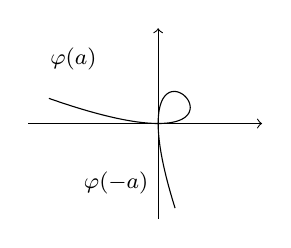
\begin{tikzpicture}[scale=1.1]
    \draw[->] (-1.5,0) -- (1.2,0);
    \draw[->] (0,-1.1) -- (0,1.1);
    \draw[smooth, samples=80, domain=-1.25:0.30] plot ({2.5*(-\x*\x*\x - 2*\x*\x - \x)}, {2.5*(\x*\x*\x + \x*\x)});
    \node[above left] at (-0.6,0.5) {\footnotesize $\varphi(a)$};
    \node[below left] at (0,-0.45) {\footnotesize $\varphi(-a)$};
\end{tikzpicture}
\end{center}

Verso? $\varphi'(0) = (-1, 0)$, $\varphi'(-1) = (0, 1)$.
\end{example}

\begin{example}[Cuspide]
$\varphi(t) = (t^3, t^2)$, $t \in [-1, 1]$.
\begin{enumerate}
    \item non è chiusa
    \item è semplice
    \item non è regolare: $\varphi'(t) = (3t^2, 2t) = (0, 0)$ se $t = 0 \implies$ non è regolare
\end{enumerate}

\begin{center}
\begin{tikzpicture}[scale=0.9]
    \draw[->] (-1.4,0) -- (1.5,0);
    \draw[->] (0,-0.4) -- (0,1.4);
    \draw[smooth, samples=60, domain=-1:1] plot ({\x*\x*\x}, {\x*\x});
\end{tikzpicture}
\end{center}
\end{example}

\begin{example}[Cicloide]
\[
\varphi : \begin{cases}
x(t) = r(t - \sin t) \\
y(t) = r(1 - \cos t)
\end{cases} \quad t \in [0, 2\pi], \ r > 0
\]

\begin{center}
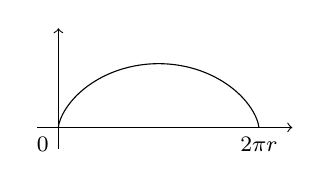
\begin{tikzpicture}[scale=0.9]
    \draw[->] (-0.3,0) -- (3.3,0);
    \draw[->] (0,-0.3) -- (0,1.4);
    \draw[smooth, samples=60, domain=0:6.2832] plot ({0.45*(\x - sin(\x r))}, {0.45*(1 - cos(\x r))});
    \node[below left] at (0,0) {\footnotesize $0$};
    \node[below] at (2.83,0) {\footnotesize $2\pi r$};
\end{tikzpicture}
\end{center}

\begin{enumerate}
    \item non è chiusa
    \item è semplice
    \item $\varphi'(t) = (1 - \cos t, \ \sin t) \cdot r$, $\vert \varphi'(t) \vert = r\sqrt{1 + \cos^2 t - 2\cos t + \sin^2 t} = r\sqrt{2}\sqrt{1 - \cos t} \neq 0$ in $]0, 2\pi[$
\end{enumerate}
\end{example}

\begin{example}[Elica $\mathbb{R}^3$]
\[
\varphi : \begin{cases}
x(t) = R \cos t \\
y(t) = R \sin t \\
z(t) = t
\end{cases} \quad t \in [0, 2\pi]
\]
\begin{enumerate}
    \item non è chiusa
    \item è semplice
    \item è regolare
\end{enumerate}

\begin{center}
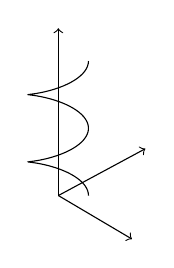
\begin{tikzpicture}[scale=0.85]
    \draw[->] (0,0) -- (0,2.5);
    \draw[->] (0,0) -- (1.3,0.7);
    \draw[->] (0,0) -- (1.1,-0.65);
    \draw[smooth, samples=100, domain=0:12.566] plot ({0.45*cos(\x r)}, {0.16*\x + 0.15*sin(\x r)});
\end{tikzpicture}
\end{center}
\end{example}

\subsection{Curve in coord. polari (\texorpdfstring{$\mathbb{R}^2$}{R 2})}

$\varphi : [a, b] \to \mathbb{R}^2$

\begin{center}
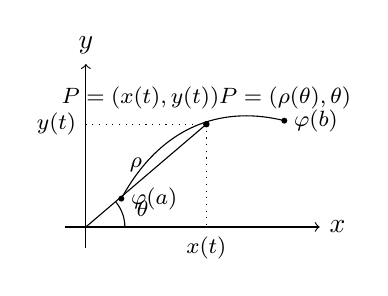
\begin{tikzpicture}[scale=0.9]
    \draw[->] (-0.3,0) -- (3.3,0) node[right] {$x$};
    \draw[->] (0,-0.3) -- (0,2.3) node[above] {$y$};
    \draw (0.5,0.4) .. controls (1.1,1.5) and (2.0,1.7) .. (2.8,1.5);
    \fill (0.5,0.4) circle (1.2pt) node[right] {\footnotesize $\varphi(a)$};
    \fill (2.8,1.5) circle (1.2pt) node[right] {\footnotesize $\varphi(b)$};
    \fill (1.7,1.45) circle (1.3pt) node[above=2pt] {\footnotesize $P = (x(t), y(t)) \implies P = (\rho(\theta), \theta )$};
    \draw (0,0) -- (1.7,1.45) node[midway, above left=-2pt] {\footnotesize $\rho$};
    \draw[dotted] (1.7,1.45) -- (1.7,0) node[below] {\footnotesize $x(t)$};
    \draw[dotted] (1.7,1.45) -- (0,1.45) node[left] {\footnotesize $y(t)$};
    \draw (0.55,0) arc (0:40:0.55);
    \node at (0.8,0.25) {\footnotesize $\theta$};
\end{tikzpicture}
\end{center}

Per il passaggio:
\[
\begin{cases}
x = \rho(\theta) \cos\theta \\
y = \rho(\theta) \sin\theta
\end{cases} \quad \theta \in [\theta_1, \theta_2]
\]

In coord. pol.:
\[
\varphi = \begin{cases}
\rho = \rho(\theta) \\
\theta = \theta
\end{cases}
\]
\pencilnote{$\to$ ($\rho$ può dip. anche da altro)}

Supp. che $\varphi$ sia assegnata nel piano polare e abbia eq.:
\[
\begin{cases}
\rho = \rho(\theta) \\
\theta = \theta
\end{cases} \quad \theta \in [\theta_1, \theta_2]
\]

\begin{center}
\begin{tikzpicture}[scale=0.8]
    \node[left, align=left] at (-0.3,1.0) {\footnotesize \pencilnote{Es.:} \\ \footnotesize \pencilnote{circonf.}};
    \draw[->] (-0.2,0) -- (2.5,0) node[right] {\footnotesize $\theta$};
    \draw[->] (0,-0.2) -- (0,1.8) node[above] {\footnotesize $\rho$};
    \draw (0,1.1) -- (1.9,1.1);
    \node[left] at (0,1.1) {\footnotesize $R$};
    \node[below left] at (0,0) {\footnotesize $0$};
    \draw[dotted] (1.9,1.1) -- (1.9,0) node[below] {\footnotesize $2\pi$};
\end{tikzpicture}
\end{center}

Sia $\rho \in C^1([\theta_1, \theta_2])$. Quali cond. deve assecondare $\rho(\theta)$ affinché $\varphi$ sia regolare?

Usando le formule di passaggio, calcolo $\varphi'(\theta)$:
\[
x'(\theta) = \rho'(\theta) \cos\theta - \rho(\theta) \sin\theta
\]
\[
y'(\theta) = \rho'(\theta) \sin\theta + \rho(\theta) \cos\theta
\]
\[
\vert \varphi'(\theta) \vert^2 = (\rho')^2 \cos^2\theta + \rho^2 \sin^2\theta + (\rho')^2 \sin^2\theta + \rho^2 \cos^2\theta - 2\rho'\rho \sin\theta \cos\theta + 2\rho'\rho \sin\theta \cos\theta = \underline{(\rho')^2 + \rho^2}
\]

\begin{prop}
Se $\varphi$ è in coord. polari
\[
\varphi : \begin{cases}
\rho = \rho(\theta) \\
\theta = \theta
\end{cases} \quad \text{con } \theta \in [\theta_1, \theta_2]
\]
Allora $\varphi$ è regolare se
\begin{enumerate}
    \item $\varphi \in C^1([\theta_1, \theta_2])$
    \item $(\rho')^2 + \rho^2 > 0 \quad \forall \theta \in ]\theta_1, \theta_2[$
\end{enumerate}
\end{prop}

\begin{example*}
\pencilnote{Exe: circonferenza in $[0, 2\pi]$

$\varphi \in C^1([0, 2\pi])$

$\rho' = 0, \ \rho^2 = R^2 \to \vert \varphi'(\theta) \vert^2 = \rho^2 \implies \vert \varphi'(\theta) \vert = \rho \implies$ è regolare}
\end{example*}

\begin{example}[Cardioide]
$\rho(\theta) = a(1 + \cos\theta)$ dove $a > 0$ fissato
\begin{itemize}
    \item $\theta \in [-\pi, \pi]$
\end{itemize}

Il sostegno è nel piano cartesiano
\[
\begin{cases}
x(\theta) = \rho(\theta) \cos\theta \\
y(\theta) = \rho(\theta) \sin\theta
\end{cases} \quad \theta \in [-\pi, \pi]
\]
\pencilnote{(è regolare; in $[0, 2\pi]$ non lo sarebbe)}

\begin{center}
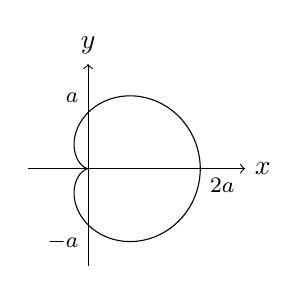
\begin{tikzpicture}[scale=0.95]
    \draw[->] (-0.8,0) -- (2.1,0) node[right] {$x$};
    \draw[->] (0,-1.3) -- (0,1.4) node[above] {$y$};
    \draw[smooth, samples=100, domain=-3.1416:3.1416] plot ({0.75*(1 + cos(\x r))*cos(\x r)}, {0.75*(1 + cos(\x r))*sin(\x r)});
    \node[above left] at (0,0.75) {\footnotesize $a$};
    \node[below left] at (0,-0.75) {\footnotesize $-a$};
    \node[below right] at (1.5,0) {\footnotesize $2a$};
\end{tikzpicture}
\end{center}

\pencilnote{Se $\theta = \pm\pi \implies \rho(\theta) = 0$; \quad $\theta = 0 \implies \rho(\theta) = 2a$; \quad $\theta = \frac{\pi}{2} \implies \rho(\theta) = a$.}

\begin{itemize}
    \item è semplice
    \item è regolare? $\rho' = -a \sin\theta \implies \vert \varphi'(\theta) \vert^2 = \underbrace{a^2 \sin^2\theta}_{(\rho')^2} + \underbrace{a^2(1 + \cos^2\theta + 2\cos\theta)}_{\rho^2} = 2a^2(1 + \cos\theta) > 0$ se $\cos\theta \neq -1$, ma $\theta \in ]-\pi, \pi[ \implies$ è vero $\implies$ è reg. in $[-\pi, \pi]$
\end{itemize}
\end{example}

\begin{example}[Spirale di Archimede]
$\rho(\theta) = a\theta$
\begin{itemize}
    \item $a > 0$, $\theta \in [0, 2\pi]$
    \item non chiusa
    \item semplice
    \item regolare
\end{itemize}

\begin{center}
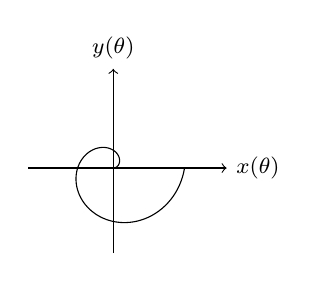
\begin{tikzpicture}[scale=0.9]
    \draw[->] (-1.2,0) -- (1.6,0) node[right] {\footnotesize $x(\theta)$};
    \draw[->] (0,-1.2) -- (0,1.4) node[above] {\footnotesize $y(\theta)$};
    \draw[smooth, samples=100, domain=0:6.2832] plot ({0.16*\x*cos(\x r)}, {0.16*\x*sin(\x r)});
\end{tikzpicture}
\end{center}
\end{example}

\[
\psi(t) = (\sqrt{1 - t^2}, t) \quad t \in \left[-\frac{\sqrt{3}}{2}, \frac{\sqrt{3}}{2}\right]
\]
\[
\gamma(t) = (\cos t, \sin t) \quad t \in \left[-\frac{\pi}{3}, \frac{\pi}{3}\right]
\]
\pencilnote{(stesso sostegno)}

\[
\varphi_1 : \begin{cases}
x = \cos t \\
y = \sin t
\end{cases} \quad t \in [0, 2\pi], \qquad
\varphi_2 : \begin{cases}
x = \cos t \\
y = \sin t
\end{cases} \quad t \in [0, 3\pi]
\]
\[
\varphi_3 : \begin{cases}
x = \cos t \\
y = -\sin t
\end{cases} \quad t \in [0, 2\pi]
\]
\pencilnote{(stesso sostegno)}

\begin{center}
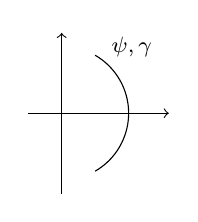
\begin{tikzpicture}[scale=0.85]
    \draw[->] (-0.5,0) -- (1.6,0);
    \draw[->] (0,-1.2) -- (0,1.2);
    \draw (0,0) ++(-60:1) arc (-60:60:1);
    \node[above right] at (0.6,0.7) {\footnotesize $\psi, \gamma$};
\end{tikzpicture}
\end{center}

\subsection{Curve equivalenti e versore tangente}

\begin{definition}
Siano $\varphi : [a, b] \to \mathbb{R}^2$ e $\psi : [c, d] \to \mathbb{R}^2$ due curve, esse si dicono \underline{eq.} se esiste $g : [a, b] \to [c, d]$ tale che:
\begin{enumerate}
    \item $g \in C^1([a, b])$
    \item $g'(t) \neq 0 \quad \forall t \in ]a, b[$ \pencilnote{($g$ è monotona e invertibile)}
    \item $\varphi(t) = \psi(g(t)) \quad \forall t \in [a, b]$
    
    $\psi(\tau) = \varphi(g^{-1}(\tau)) \quad \forall \tau \in [c, d]$ dato $g^{-1}$ esiste per (2).
\end{enumerate}
$g$ prende il nome di \underline{diffeomorfismo} o \underline{cambiamento ammissibile di parametro} e scriveremo $\varphi \sim \psi$.
\end{definition}

Si dim. che $\sim$ è una \underline{relazione d'eq.}

\begin{example}
$\psi(t) = (\sqrt{1 - t^2}, t) \quad t \in \left[-\frac{\sqrt{3}}{2}, \frac{\sqrt{3}}{2}\right]$

$\gamma(t) = (\cos t, \sin t) \quad t \in \left[-\frac{\pi}{3}, \frac{\pi}{3}\right]$

\begin{center}
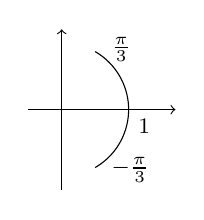
\begin{tikzpicture}[scale=0.85]
    \draw[->] (-0.5,0) -- (1.7,0);
    \draw[->] (0,-1.2) -- (0,1.2);
    \draw (0,0) ++(-60:1) arc (-60:60:1);
    \node[below right] at (1,0) {\footnotesize $1$};
    \node[right] at (0.6,0.9) {\footnotesize $\frac{\pi}{3}$};
    \node[right] at (0.6,-0.9) {\footnotesize $-\frac{\pi}{3}$};
\end{tikzpicture}
\end{center}

Mi domando:
\[
\exists g : \left[-\frac{\pi}{3}, \frac{\pi}{3}\right] \to \left[-\frac{\sqrt{3}}{2}, \frac{\sqrt{3}}{2}\right] \text{ tale che: } \psi(g(t)) = \gamma(t)
\]
\[
(\cos t, \sin t) = (\sqrt{1 - g^2(t)}, g(t)) \implies \begin{cases}
\sin(t) = g(t) \\
\cos t = \sqrt{1 - \sin^2 t} = \vert \cos t \vert = \cos t \quad t \in \left[-\frac{\pi}{3}, \frac{\pi}{3}\right]
\end{cases}
\]
\[
g'(t) = \cos t > 0 \quad \text{per } t \in \left[-\frac{\pi}{3}, \frac{\pi}{3}\right]
\]
\end{example}

\[
\varphi_1 = \begin{cases}
x = \cos t \\
y = \sin t
\end{cases} \quad t \in [0, 2\pi] \qquad
\varphi_2 = \begin{cases}
x = \cos t \\
y = -\sin t
\end{cases} \quad t \in [0, 2\pi]
\]

\begin{center}
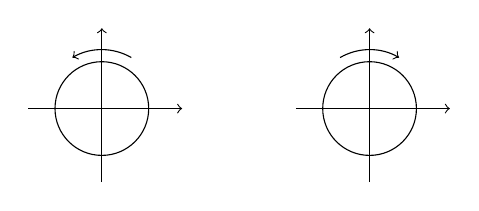
\begin{tikzpicture}[scale=0.85]
    % Cerchio phi_1 (antiorario)
    \draw[->] (-1.1,0) -- (1.2,0);
    \draw[->] (0,-1.1) -- (0,1.2);
    \draw (0,0) circle (0.7);
    \draw[->] (60:0.88) arc (60:120:0.88);

    % Cerchio phi_2 (orario)
    \begin{scope}[xshift=4cm]
        \draw[->] (-1.1,0) -- (1.2,0);
        \draw[->] (0,-1.1) -- (0,1.2);
        \draw (0,0) circle (0.7);
        \draw[->] (120:0.88) arc (120:60:0.88);
    \end{scope}
\end{tikzpicture}
\end{center}

\[
g(t) = -t + 2\pi
\]
\[
\varphi_2(g(t)) = \varphi_2(-t + 2\pi) = (\cos t, \sin t) = \varphi_1(t)
\]

\begin{oss}
Il verso di percorrenza è superfluo ai fini dell'equivalenza.
\end{oss}

\begin{definition}
\underline{``Verso di percorrenza''}: $P = \varphi(t_1)$ ``precede'' $Q = \varphi(t_2)$ se $t_1 < t_2$.
\end{definition}

\begin{definition}
$\varphi \stackrel{\circ}{\sim} \psi$ se $\varphi \sim \psi$ e $g' > 0$ \pencilnote{(equivalenti con stesso verso di percorrenza)}.
\end{definition}

\begin{prop}
Siano $\varphi : [a, b] \to \mathbb{R}^2$ e $\psi : [c, d] \to \mathbb{R}^2$ due curve equivalenti $\varphi \sim \psi$.

Se le curve hanno lo stesso orientamento \pencilnote{($\stackrel{\circ}{\sim}$)}, allora hanno lo stesso versore tangente, altrimenti sono opposti.
\end{prop}

\begin{proof}
$\varphi \sim \psi \implies \exists g : [a, b] \to [c, d]$ diffeomorfismo \pencilnote{($g' > 0$ o $g' < 0$)} tale che $\varphi(t) = \psi(g(t))$.

Sia $t_0 \in [a, b]$, calc. il vers. tang.: $T_\varphi(t_0)$.

Sia $P_0 = \varphi(t_0)$ e sia $\tau_0 : g(t_0) = \tau_0$ e $P_0 = \psi(\tau_0)$
\[
T_\varphi(t_0) = \frac{\varphi'(t_0)}{\vert \varphi'(t_0) \vert} = \frac{\frac{d}{dt}(\psi(g(t)))}{\left\vert \frac{d}{dt}(\psi(g(t))) \right\vert} \Bigg|_{t = t_0} = \frac{\psi'(\overbrace{g(t_0)}^{\tau_0}) g'(t_0)}{\vert \psi'(\underbrace{g(t_0)}_{\tau_0}) \vert \, \vert g'(t_0) \vert} = T_\psi(\tau_0) \frac{g'(t_0)}{\vert g'(t_0) \vert}
\]
\pencilnote{(dove $\frac{g'(t_0)}{\vert g'(t_0) \vert}$ vale $+1$ oppure $-1$)}.
\end{proof}

\subsection{Lunghezza di una curva}

$\varphi : [a, b] \to \mathbb{R}^2$

$t_0 = a < t_1 < t_2 < \dots < t_k = b$

\begin{center}
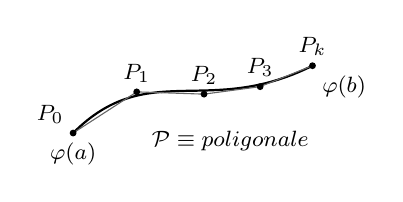
\begin{tikzpicture}[scale=0.95]
    \draw[thick] (0,0.2) .. controls (1.0,1.2) and (1.8,0.4) .. (3.2,1.1);
    \coordinate (P0) at (0,0.2);
    \coordinate (P1) at (0.85,0.75);
    \coordinate (P2) at (1.75,0.72);
    \coordinate (P3) at (2.5,0.82);
    \coordinate (Pk) at (3.2,1.1);
    \draw[gray!80!black] (P0) -- (P1) -- (P2) -- (P3) -- (Pk);
    \fill (P0) circle (1.3pt) node[above left] {\footnotesize $P_0$} node[below] {\footnotesize \pencilnote{$\varphi(a)$}};
    \fill (P1) circle (1.3pt) node[above] {\footnotesize $P_1$};
    \fill (P2) circle (1.3pt) node[above] {\footnotesize $P_2$};
    \fill (P3) circle (1.3pt) node[above] {\footnotesize $P_3$};
    \fill (Pk) circle (1.3pt) node[above] {\footnotesize $P_k$} node[below right] {\footnotesize \pencilnote{$\varphi(b)$}};
    \node[below] at (2.1,0.35) {\footnotesize $\mathcal{P} \equiv \text{poligonale}$};
\end{tikzpicture}
\end{center}

$\implies P_i = \varphi(t_i) \implies P_0 = \varphi(a), \ P_1 = \varphi(t_1), \ \dots, \ P_k = \varphi(b)$
\[
\begin{aligned}
l(\mathcal{P}) &= \underbrace{\vert P_0 - P_1 \vert}_{\text{lunghezza del segmento}} + \vert P_1 - P_2 \vert + \dots + \vert P_{k-1} - P_k \vert > 0 \\
&= \sqrt{(x_0 - x_1)^2 + (y_0 - y_1)^2} + \dots + \sqrt{(x_{k-1} - x_k)^2 + (y_{k-1} - y_k)^2} \\
&= \sum_{i=1}^{k} \vert \varphi(t_i) - \varphi(t_{i-1}) \vert = \sum_{i=1}^{k} \sqrt{(x(t_i) - x(t_{i-1}))^2 + (y(t_i) - y(t_{i-1}))^2}
\end{aligned}
\]
\pencilnote{(dove $P_i = (x_i, y_i) = (x(t_i), y(t_i))$)}.

Per def.: \underline{lunghezza di $\varphi$}:
\[
l(\varphi) = \sup \{ l(\mathcal{P}), \ \mathcal{P} \text{ spezzata} \}
\]
Diremo che la curva $\varphi$ è ``rettificabile'' se $l(\varphi)$ è finita, $l(\varphi) < +\infty$.

\begin{theorem}[Teo di rettificabilità (SD)]
Sia $\varphi : [a, b] \to \mathbb{R}^2$ una curva \underline{regolare}.

Allora $\varphi$ è \underline{rettificabile} e si ha che
\[
l(\varphi) = \int_a^b \vert \varphi'(t) \vert \, dt
\]
\end{theorem}

Perimetro: se $\varphi$ è semplice, esso è uguale a $l(\varphi)$.

\begin{prop}
Se $\gamma$ e $\psi$ sono due curve regolari con $\gamma : [a, b] \to \mathbb{R}^2$ e $\psi : [c, d] \to \mathbb{R}^2$.

Se $\gamma \sim \psi$ allora $l(\gamma) = l(\psi)$
\end{prop}

\begin{proof}
Sia $g$ un diff., $g : [a, b] \to [c, d]$ e $\gamma(t) = \psi(g(t))$ $t \in [a, b]$.

Per il teo di rettificabilità: $l(\gamma) = \int_a^b \vert \gamma'(t) \vert \, dt$ e $l(\psi) = \int_c^d \vert \psi'(\tau) \vert \, d\tau$. Dim. che coincidono:
\[
l(\gamma) = \int_a^b \vert \psi'(g(t)) \vert \, \vert g'(t) \vert \, dt =
\]
Se pongo $g(t) = \tau$ allora $g'(t) \, dt = d\tau$
\[
= \int \vert \psi'(\tau) \vert \frac{\vert g'(t) \vert}{g'(t)} \, d\tau = \begin{cases}
g' > 0 \to \int_c^d \vert \psi'(\tau) \vert \, d\tau \\
g' < 0 \to -\int_d^c \vert \psi'(\tau) \vert \, d\tau = \int_c^d \vert \psi'(\tau) \vert \, d\tau
\end{cases}
\]
\end{proof}

\begin{example}
\[
f(x) = \begin{cases}
0 & \text{se } x = 0 \\
x \sin\left(\frac{\pi}{2x}\right) & 0 < x \le 1
\end{cases}
\]
$f : [0, 1] \to \mathbb{R}$, $f \in C^0([0, 1])$ non $C^1$.

$\gamma(t) = (t, f(t))$

$t_0 = 1 > \dots > t_i = \frac{1}{2i+1} > \dots > t_{k-1} = \frac{1}{2k-1} > t_k = 0$ \pencilnote{($\to$ sfrutto parità di varie $f_i$)}

$P_i = (t_i, f(t_i)) = \left(t_i, t_i \sin\left(\frac{\pi}{2t_i}\right)\right)$

Allora $l(\mathcal{P}) > \sum_{i=1}^{k} \frac{1}{i}$

\begin{center}
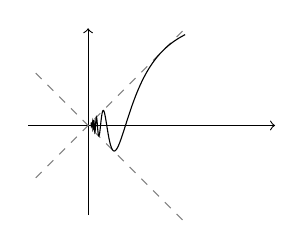
\begin{tikzpicture}[scale=0.95]
    \draw[->] (-0.8,0) -- (2.5,0);
    \draw[->] (0,-1.2) -- (0,1.3);
    \draw[dashed, gray] (-0.7,-0.7) -- (1.3,1.3);
    \draw[dashed, gray] (-0.7,0.7) -- (1.3,-1.3);
    \draw[smooth, samples=250, domain=0.04:1.3] plot (\x, {\x * sin(90/\x)});
\end{tikzpicture}
\end{center}
\end{example}

$\gamma : [a, b] \to \mathbb{R}^2$ regolare
\[
s(t) : t \in [a, b] \to \int_a^t \vert \gamma'(\tau) \vert \, d\tau = s(t) \in [0, l(\gamma)]
\]

\begin{center}
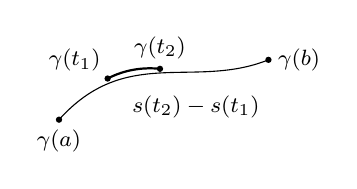
\begin{tikzpicture}[scale=0.95]
    \draw (0,0.2) .. controls (0.9,1.2) and (1.8,0.6) .. (2.8,1.0);
    \fill (0,0.2) circle (1.2pt) node[below] {\footnotesize $\gamma(a)$};
    \fill (2.8,1.0) circle (1.2pt) node[right] {\footnotesize $\gamma(b)$};
    \fill (0.65,0.75) circle (1.2pt) node[above left=-1pt] {\footnotesize $\gamma(t_1)$};
    \fill (1.35,0.88) circle (1.2pt) node[above] {\footnotesize $\gamma(t_2)$};
    \draw[thick] (0.65,0.75) .. controls (0.9,0.88) and (1.15,0.9) .. (1.35,0.88);
    \node[below right] at (0.85,0.65) {\footnotesize $s(t_2) - s(t_1)$};
\end{tikzpicture}
\end{center}

\begin{enumerate}
    \item $s(t) : [a, b] \to [0, l(\gamma)]$ \pencilnote{($c = 0, \ d = l(\gamma)$)}
    \item $s(t) \in C^1([a, b])$ e $s'(t) = \vert \gamma'(t) \vert$ \pencilnote{(teo fond. c. int.)}
    \item $s'(t) \neq 0 \quad t \in ]a, b[$ \pencilnote{($\leftarrow$ per regolarità)}
\end{enumerate}

\underline{Definisco} $\psi : [0, l(\gamma)] \to \mathbb{R}^2$, $\psi(\tau) = \gamma(s^{-1}(\tau))$

Per costruzione $\gamma \sim \psi$

$s$ si chiama \underline{ascissa curvilinea} o \underline{lunghezza d'arco} \pencilnote{(è un diffeomorfismo)}.
\[
\psi'(\tau) = \gamma'(s^{-1}(\tau)) \cdot \frac{1}{s'(s^{-1}(\tau))} = \frac{\gamma'(s^{-1}(\tau))}{\vert \gamma'(s^{-1}(\tau)) \vert} \quad \text{\pencilnote{è un versore}}
\]
Posso dire che $\underbrace{\vert \gamma'(t) \vert}_{\frac{ds}{dt}} \, dt = ds$

\subsection{Versore normale}

Vers. tang. ruotato di $\frac{\pi}{2}$ in verso \underline{orario}.

\underline{Per le superfici lo prendiamo che punta verso ``fuori''}.

\begin{center}
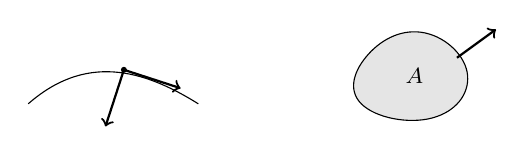
\begin{tikzpicture}[scale=0.9]
    % Curva con versore tangente e normale
    \draw (0,0.4) .. controls (0.8,1.1) and (1.6,0.9) .. (2.4,0.4);
    \coordinate (P) at (1.35,0.88);
    \fill (P) circle (1.2pt);
    \draw[->, thick] (P) -- (2.15,0.62);
    \draw[->, thick] (P) -- (1.09,0.08);

    % Superficie A con normale esterna
    \begin{scope}[xshift=4.5cm, yshift=0.1cm]
        \filldraw[fill=gray!20, draw=black] plot[smooth cycle, tension=0.8] coordinates {(0.2,0.3) (1.2,0.1) (1.7,0.7) (1.1,1.3) (0.3,1.0)};
        \node at (0.95,0.7) {\footnotesize $A$};
        \draw[->, thick] (1.55,0.95) -- (2.1,1.35);
    \end{scope}
\end{tikzpicture}
\end{center}
\[
N(t) = \frac{(y'(t), -x'(t))}{\sqrt{x'(t)^2 + y'(t)^2}}
\]
